% Auto-generated by `python new.py summarize` on 2026-06-10T10:36:21.
% Folder: experiments/2026-06-10_u_axes/
% Paste into a beamer document. Adjust the graphicspath or paths below if compiling from a different working directory.
%
% Requires: \usepackage{graphicx}

\begin{frame}{Llama-3.2-1B\_n0\_current --- Layer×layer CKA: U vs P\_U and U vs I}
  \begin{center}
    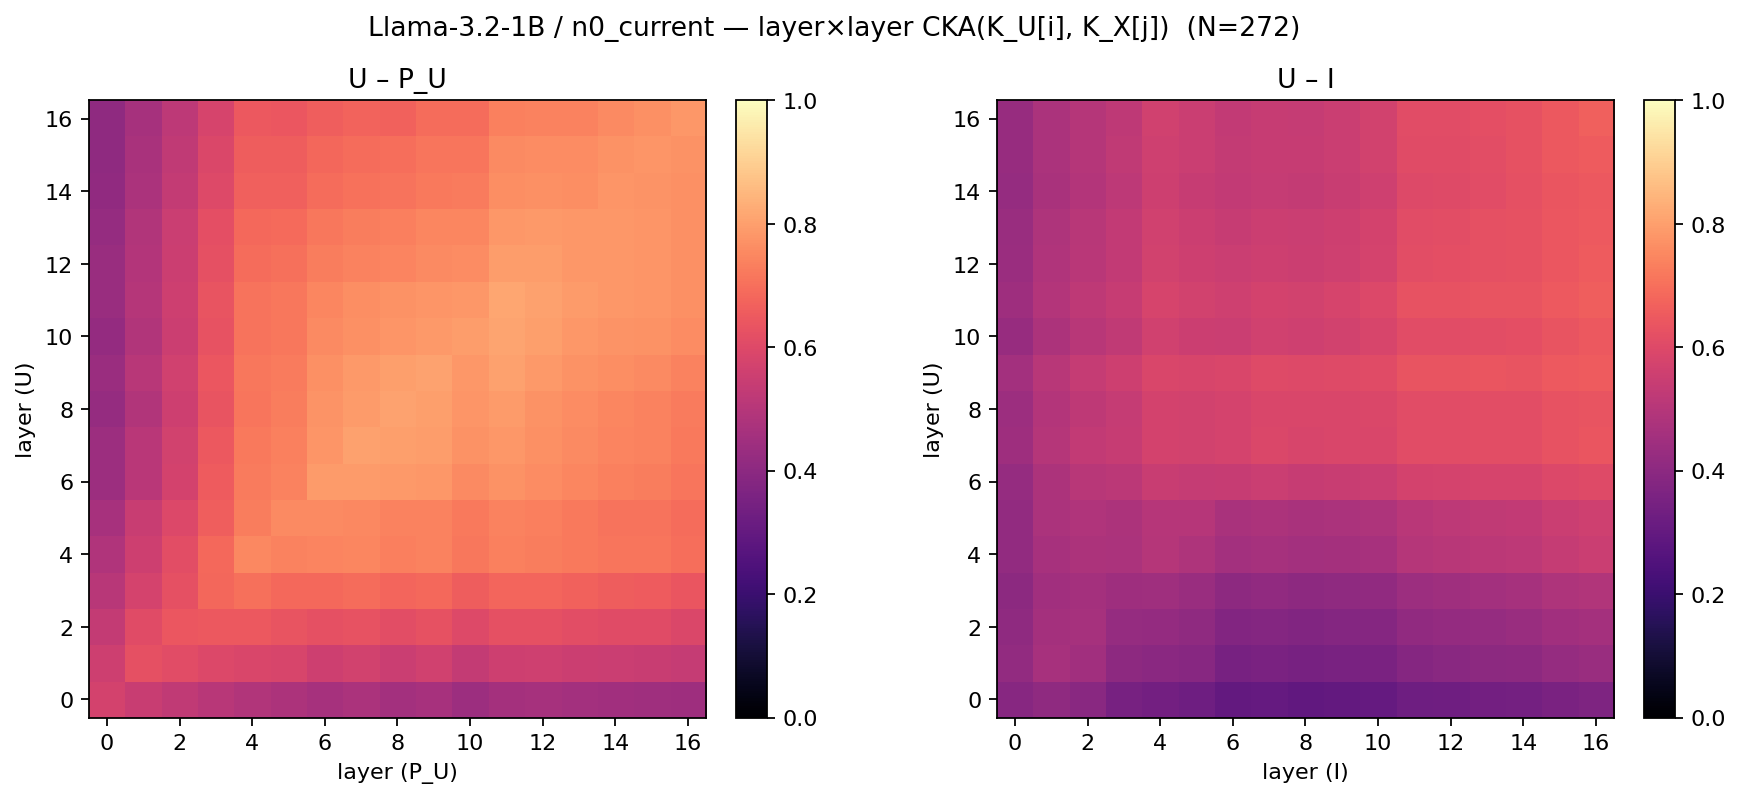
\includegraphics[width=0.95\textwidth,height=0.82\textheight,keepaspectratio]{experiments/2026-06-10_u_axes/plots/Llama-3.2-1B_n0_current/u_axes_layer_vs_layer.png}
  \end{center}
\end{frame}

\begin{frame}{Llama-3.2-1B\_n0\_current --- Layer×layer CKA: U vs P\_U and U vs I}
  \small
  \textbf{Computation.} Left: $M_{P_U}[i,j] = \mathrm{CKA}(K_U[i], K_{P_U}[j])$. Right: same with $K_I$. Diagonal cells reproduce the within-layer curves; off-diagonals are cross-depth alignment.
  \par\vspace{0.8em}
  \textbf{Interpretation.} Off-diagonal brightness flags delayed binding: $U$'s geometry at layer $i$ already matches the other bracket's geometry at a different layer $j$. Diagonal block structure suggests depth stages over which the alignment stabilizes.
\end{frame}

\begin{frame}{Llama-3.2-1B\_n0\_current --- U–P\_U and U–I across layers}
  \begin{center}
    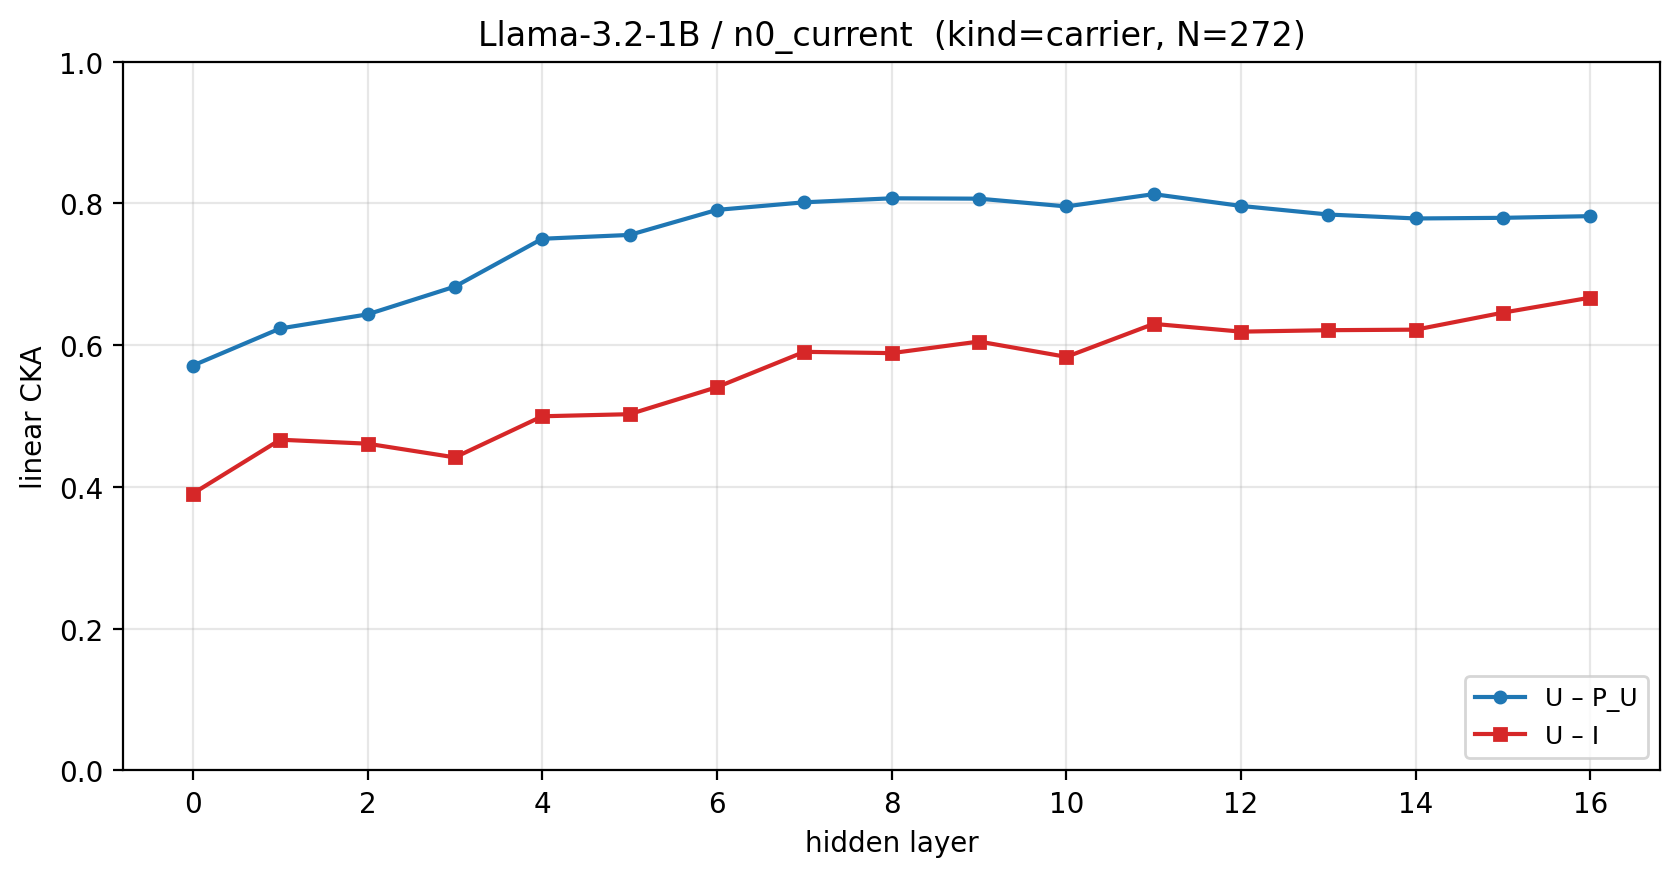
\includegraphics[width=0.95\textwidth,height=0.82\textheight,keepaspectratio]{experiments/2026-06-10_u_axes/plots/Llama-3.2-1B_n0_current/u_axes_pPU_pI.png}
  \end{center}
\end{frame}

\begin{frame}{Llama-3.2-1B\_n0\_current --- U–P\_U and U–I across layers}
  \small
  \textbf{Computation.} For each hidden layer $L$, build centered Gram matrices $K_X = X_c X_c^{\!\top}$ ($X_c = X - \bar X$) from the per-row bracket embeddings $X \in \{U, P_U, I\}$ over the $N$ stimuli. Plot linear CKA $\langle K_U, K_X\rangle_F / (\|K_U\|_F\,\|K_X\|_F)$ vs $L$ for each pair.
  \par\vspace{0.8em}
  \textbf{Interpretation.} How aligned the answer's geometry is with the paraphrase ($P_U$) and the inference ($I$) at each depth — higher means the two brackets reorder stimuli the same way. Where the two curves cross and how the gap evolves reveal when the model commits to a semantic vs pragmatic binding.
\end{frame}

\begin{frame}{Llama-3.2-1B\_p5\_fwd --- Layer×layer CKA: U vs P\_U and U vs I}
  \begin{center}
    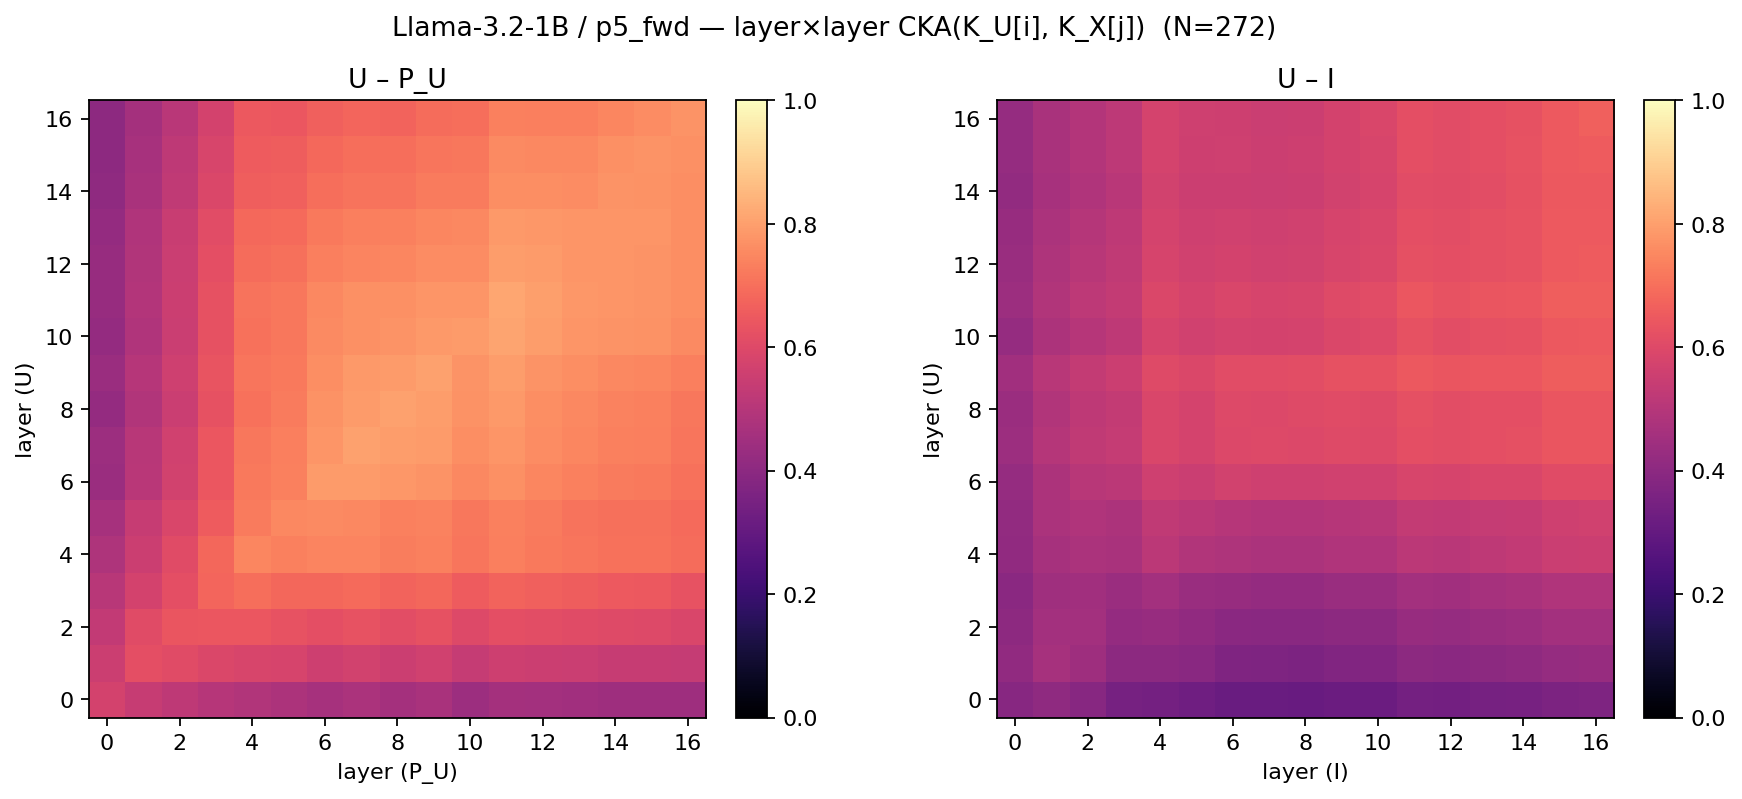
\includegraphics[width=0.95\textwidth,height=0.82\textheight,keepaspectratio]{experiments/2026-06-10_u_axes/plots/Llama-3.2-1B_p5_fwd/u_axes_layer_vs_layer.png}
  \end{center}
\end{frame}

\begin{frame}{Llama-3.2-1B\_p5\_fwd --- Layer×layer CKA: U vs P\_U and U vs I}
  \small
  \textbf{Computation.} Left: $M_{P_U}[i,j] = \mathrm{CKA}(K_U[i], K_{P_U}[j])$. Right: same with $K_I$. Diagonal cells reproduce the within-layer curves; off-diagonals are cross-depth alignment.
  \par\vspace{0.8em}
  \textbf{Interpretation.} Off-diagonal brightness flags delayed binding: $U$'s geometry at layer $i$ already matches the other bracket's geometry at a different layer $j$. Diagonal block structure suggests depth stages over which the alignment stabilizes.
\end{frame}

\begin{frame}{Llama-3.2-1B\_p5\_fwd --- U–P\_U and U–I across layers}
  \begin{center}
    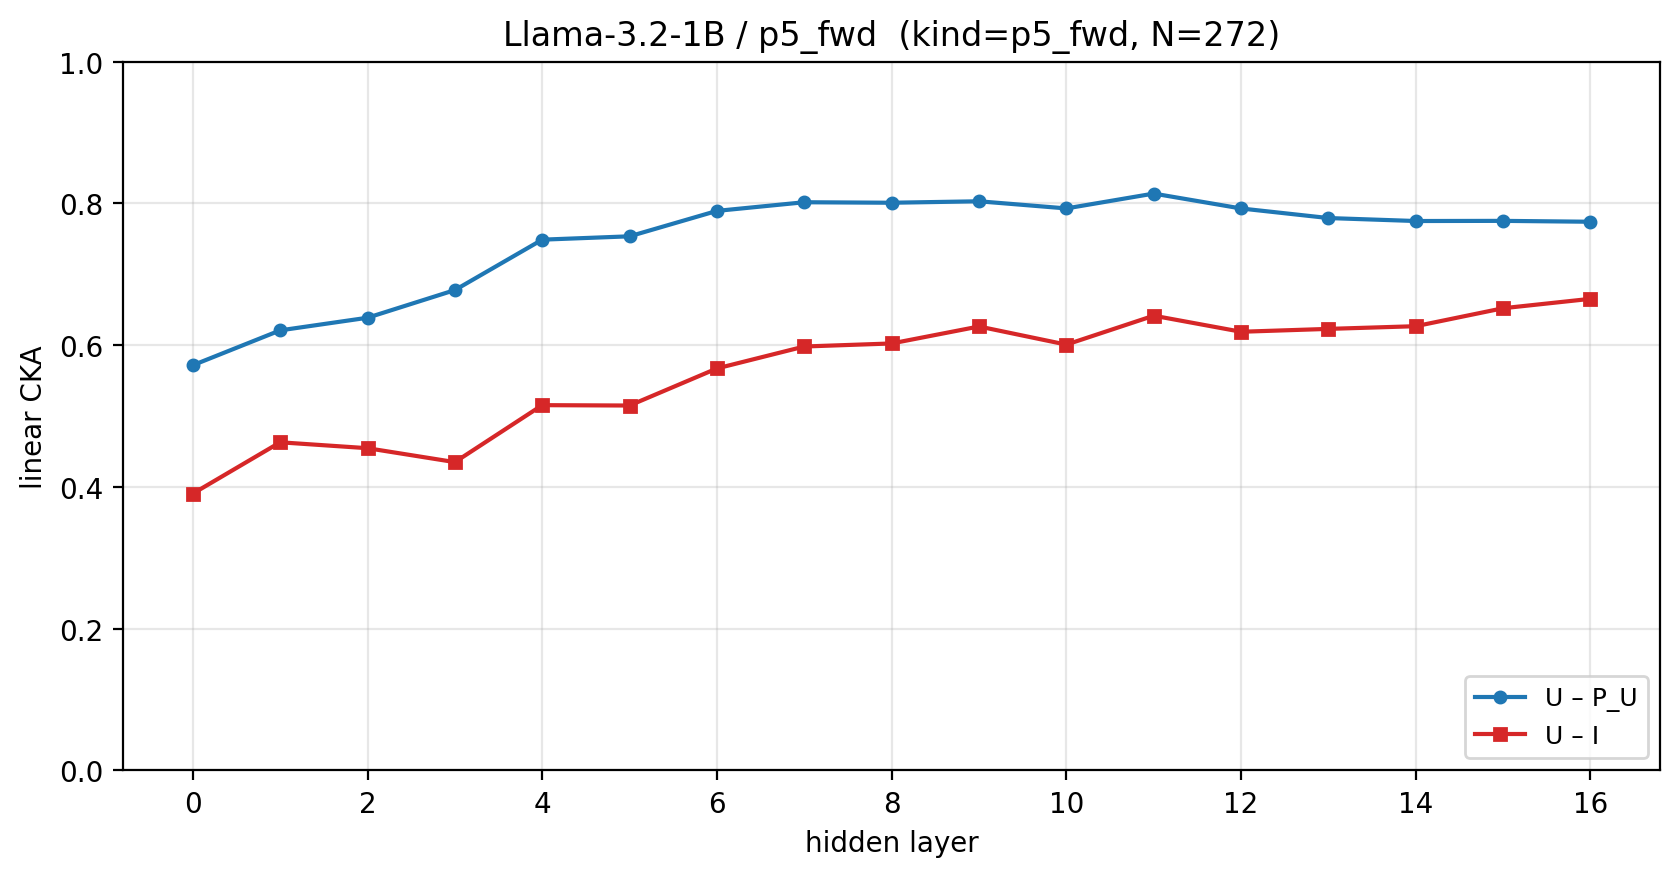
\includegraphics[width=0.95\textwidth,height=0.82\textheight,keepaspectratio]{experiments/2026-06-10_u_axes/plots/Llama-3.2-1B_p5_fwd/u_axes_pPU_pI.png}
  \end{center}
\end{frame}

\begin{frame}{Llama-3.2-1B\_p5\_fwd --- U–P\_U and U–I across layers}
  \small
  \textbf{Computation.} For each hidden layer $L$, build centered Gram matrices $K_X = X_c X_c^{\!\top}$ ($X_c = X - \bar X$) from the per-row bracket embeddings $X \in \{U, P_U, I\}$ over the $N$ stimuli. Plot linear CKA $\langle K_U, K_X\rangle_F / (\|K_U\|_F\,\|K_X\|_F)$ vs $L$ for each pair.
  \par\vspace{0.8em}
  \textbf{Interpretation.} How aligned the answer's geometry is with the paraphrase ($P_U$) and the inference ($I$) at each depth — higher means the two brackets reorder stimuli the same way. Where the two curves cross and how the gap evolves reveal when the model commits to a semantic vs pragmatic binding.
\end{frame}

\begin{frame}{Llama-3.2-1B\_p5\_rev --- Layer×layer CKA: U vs P\_U and U vs I}
  \begin{center}
    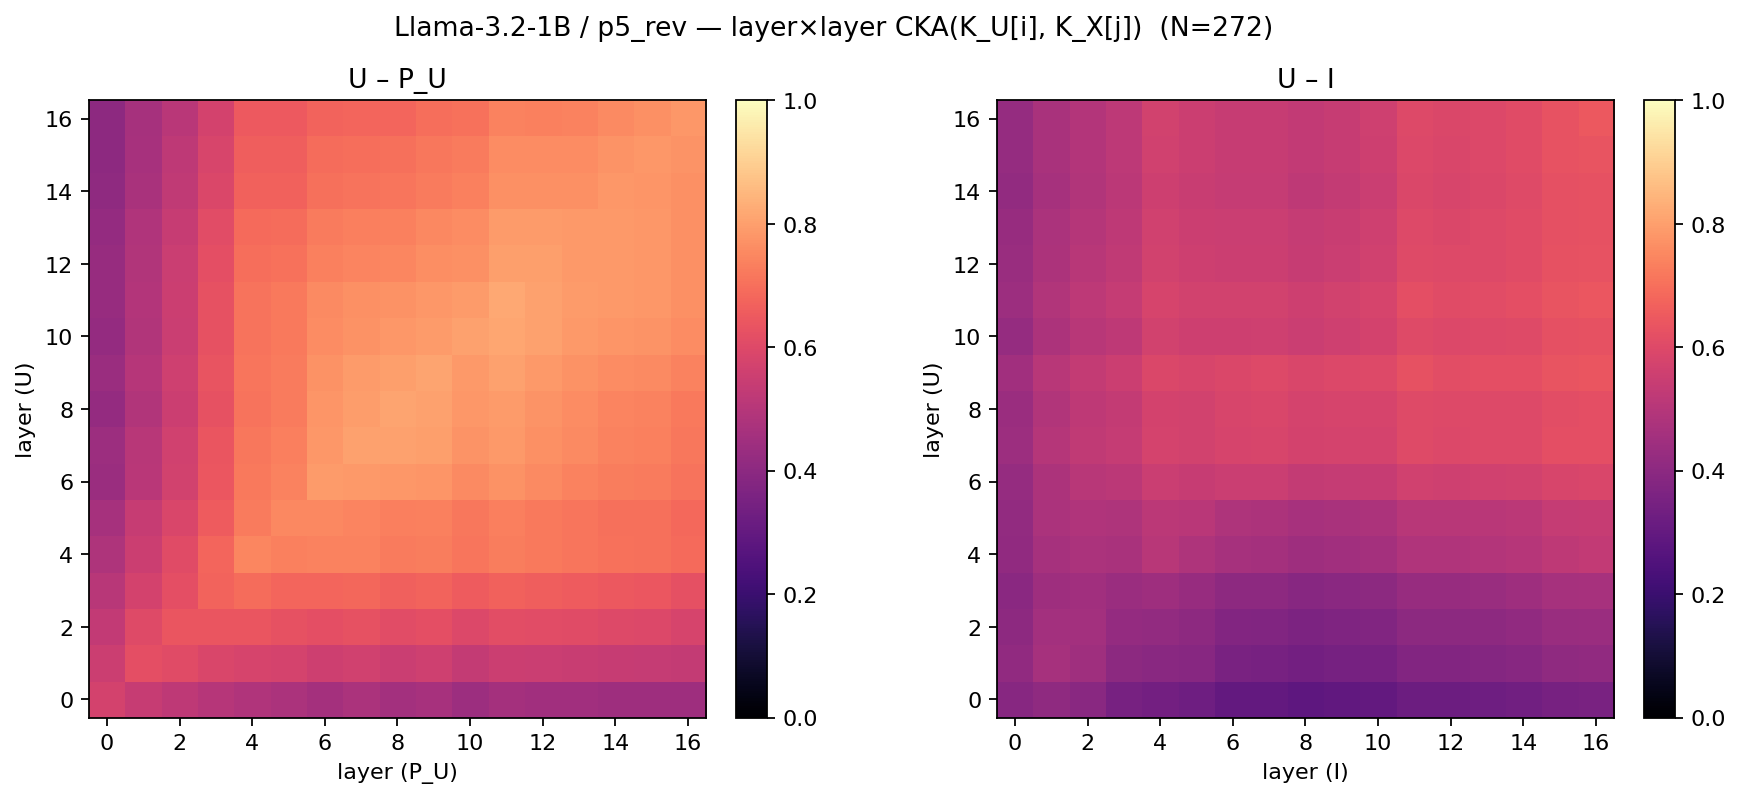
\includegraphics[width=0.95\textwidth,height=0.82\textheight,keepaspectratio]{experiments/2026-06-10_u_axes/plots/Llama-3.2-1B_p5_rev/u_axes_layer_vs_layer.png}
  \end{center}
\end{frame}

\begin{frame}{Llama-3.2-1B\_p5\_rev --- Layer×layer CKA: U vs P\_U and U vs I}
  \small
  \textbf{Computation.} Left: $M_{P_U}[i,j] = \mathrm{CKA}(K_U[i], K_{P_U}[j])$. Right: same with $K_I$. Diagonal cells reproduce the within-layer curves; off-diagonals are cross-depth alignment.
  \par\vspace{0.8em}
  \textbf{Interpretation.} Off-diagonal brightness flags delayed binding: $U$'s geometry at layer $i$ already matches the other bracket's geometry at a different layer $j$. Diagonal block structure suggests depth stages over which the alignment stabilizes.
\end{frame}

\begin{frame}{Llama-3.2-1B\_p5\_rev --- U–P\_U and U–I across layers}
  \begin{center}
    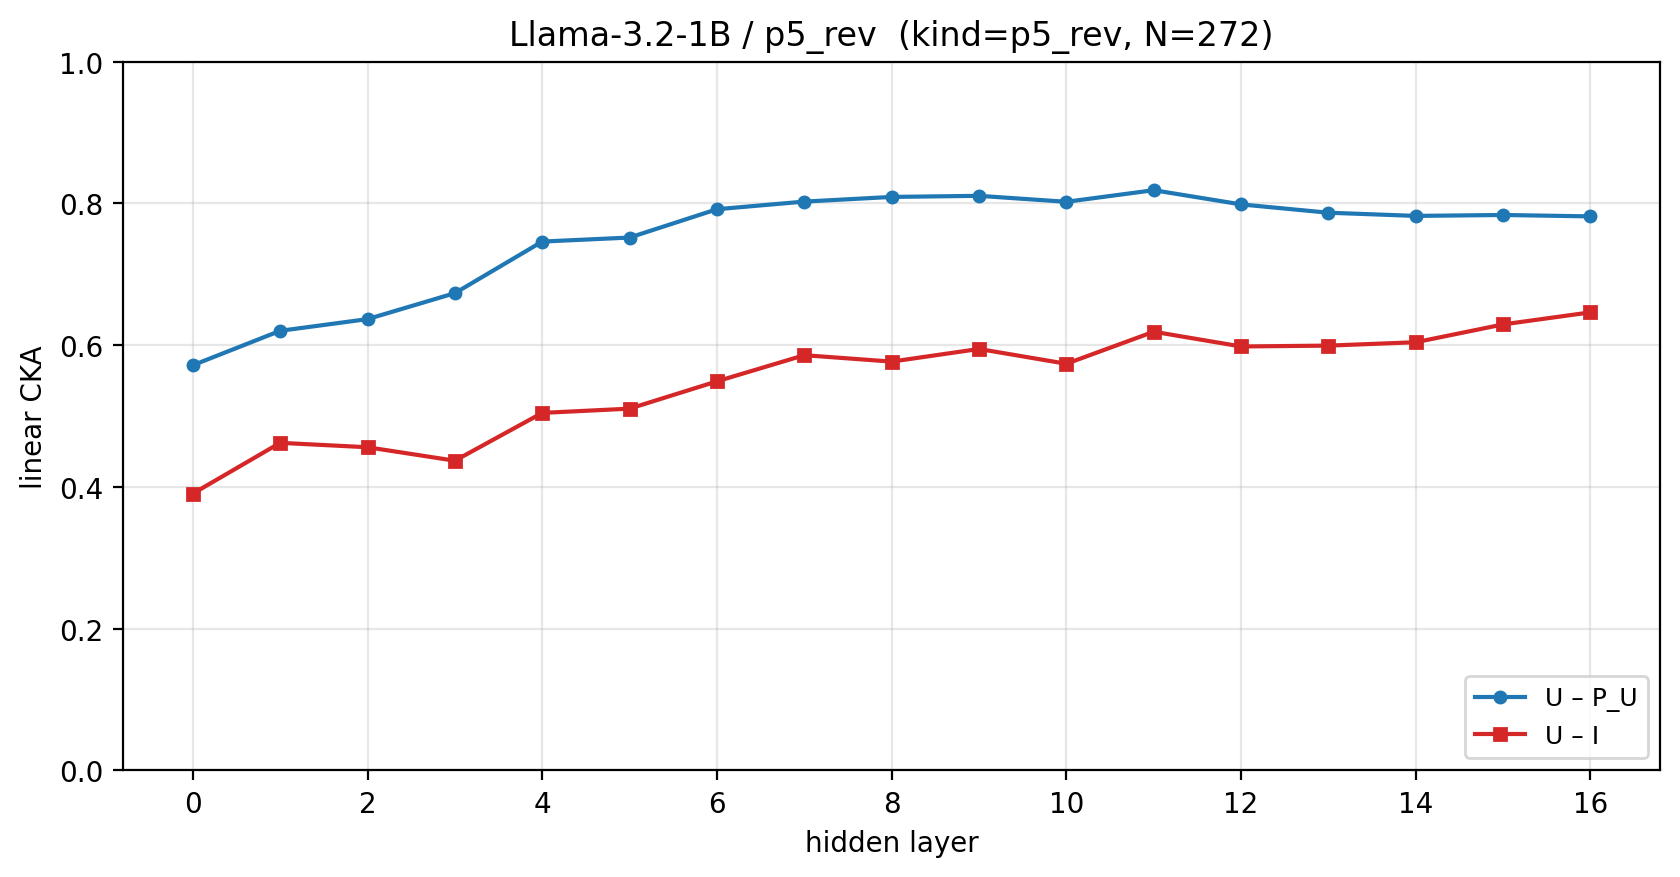
\includegraphics[width=0.95\textwidth,height=0.82\textheight,keepaspectratio]{experiments/2026-06-10_u_axes/plots/Llama-3.2-1B_p5_rev/u_axes_pPU_pI.png}
  \end{center}
\end{frame}

\begin{frame}{Llama-3.2-1B\_p5\_rev --- U–P\_U and U–I across layers}
  \small
  \textbf{Computation.} For each hidden layer $L$, build centered Gram matrices $K_X = X_c X_c^{\!\top}$ ($X_c = X - \bar X$) from the per-row bracket embeddings $X \in \{U, P_U, I\}$ over the $N$ stimuli. Plot linear CKA $\langle K_U, K_X\rangle_F / (\|K_U\|_F\,\|K_X\|_F)$ vs $L$ for each pair.
  \par\vspace{0.8em}
  \textbf{Interpretation.} How aligned the answer's geometry is with the paraphrase ($P_U$) and the inference ($I$) at each depth — higher means the two brackets reorder stimuli the same way. Where the two curves cross and how the gap evolves reveal when the model commits to a semantic vs pragmatic binding.
\end{frame}

\begin{frame}{Qwen2.5-0.5B-Instruct\_p5\_fwd --- Layer×layer CKA: U vs P\_U and U vs I}
  \begin{center}
    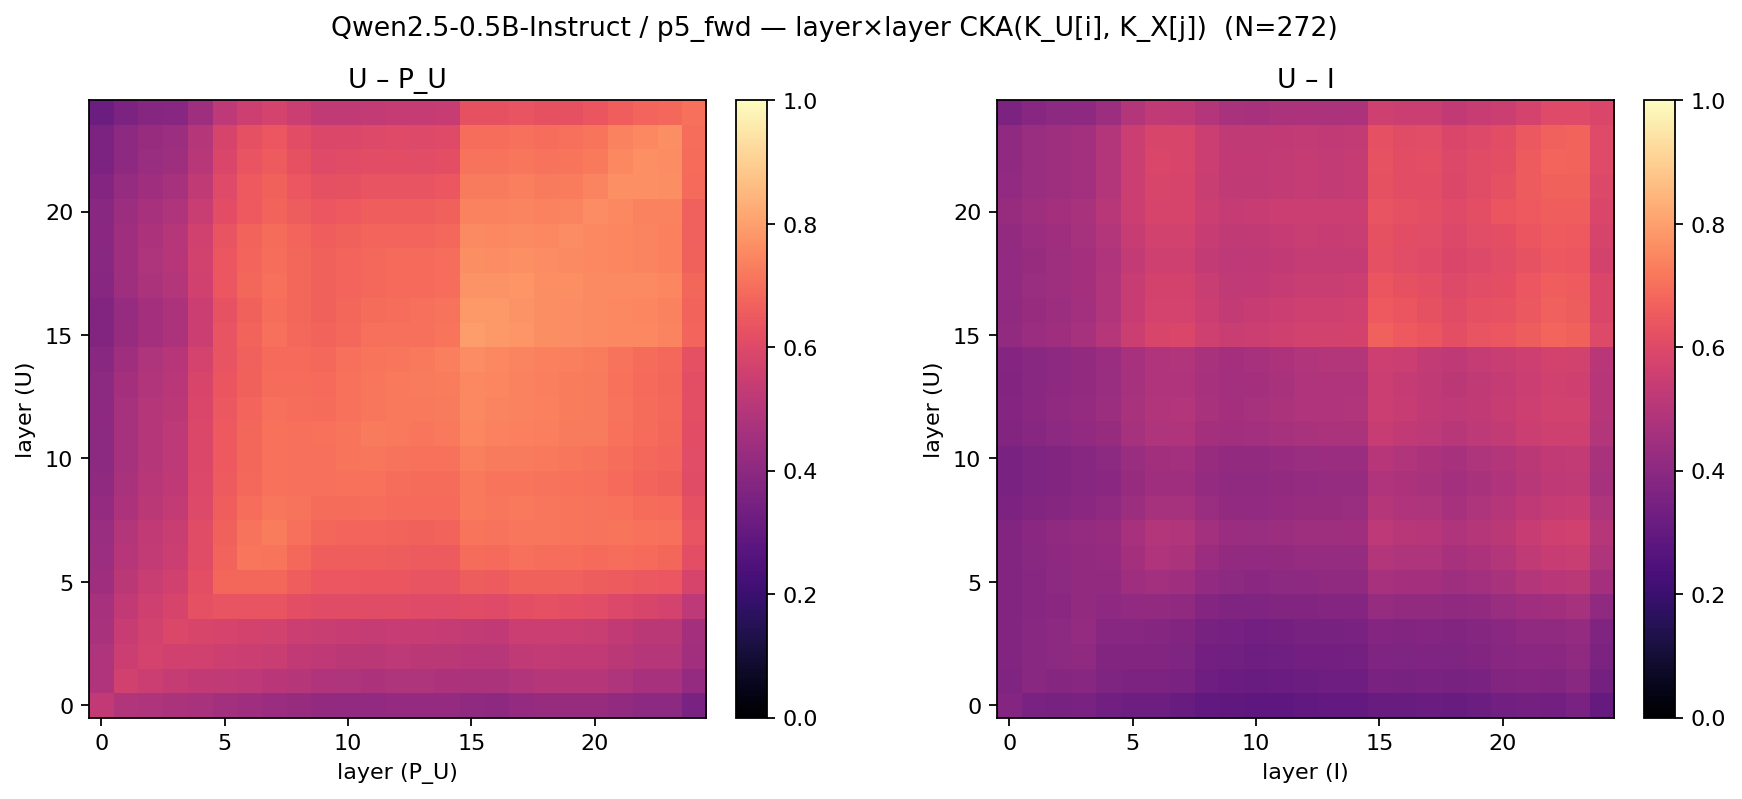
\includegraphics[width=0.95\textwidth,height=0.82\textheight,keepaspectratio]{experiments/2026-06-10_u_axes/plots/Qwen2.5-0.5B-Instruct_p5_fwd/u_axes_layer_vs_layer.png}
  \end{center}
\end{frame}

\begin{frame}{Qwen2.5-0.5B-Instruct\_p5\_fwd --- Layer×layer CKA: U vs P\_U and U vs I}
  \small
  \textbf{Computation.} Left: $M_{P_U}[i,j] = \mathrm{CKA}(K_U[i], K_{P_U}[j])$. Right: same with $K_I$. Diagonal cells reproduce the within-layer curves; off-diagonals are cross-depth alignment.
  \par\vspace{0.8em}
  \textbf{Interpretation.} Off-diagonal brightness flags delayed binding: $U$'s geometry at layer $i$ already matches the other bracket's geometry at a different layer $j$. Diagonal block structure suggests depth stages over which the alignment stabilizes.
\end{frame}

\begin{frame}{Qwen2.5-0.5B-Instruct\_p5\_fwd --- U–P\_U and U–I across layers}
  \begin{center}
    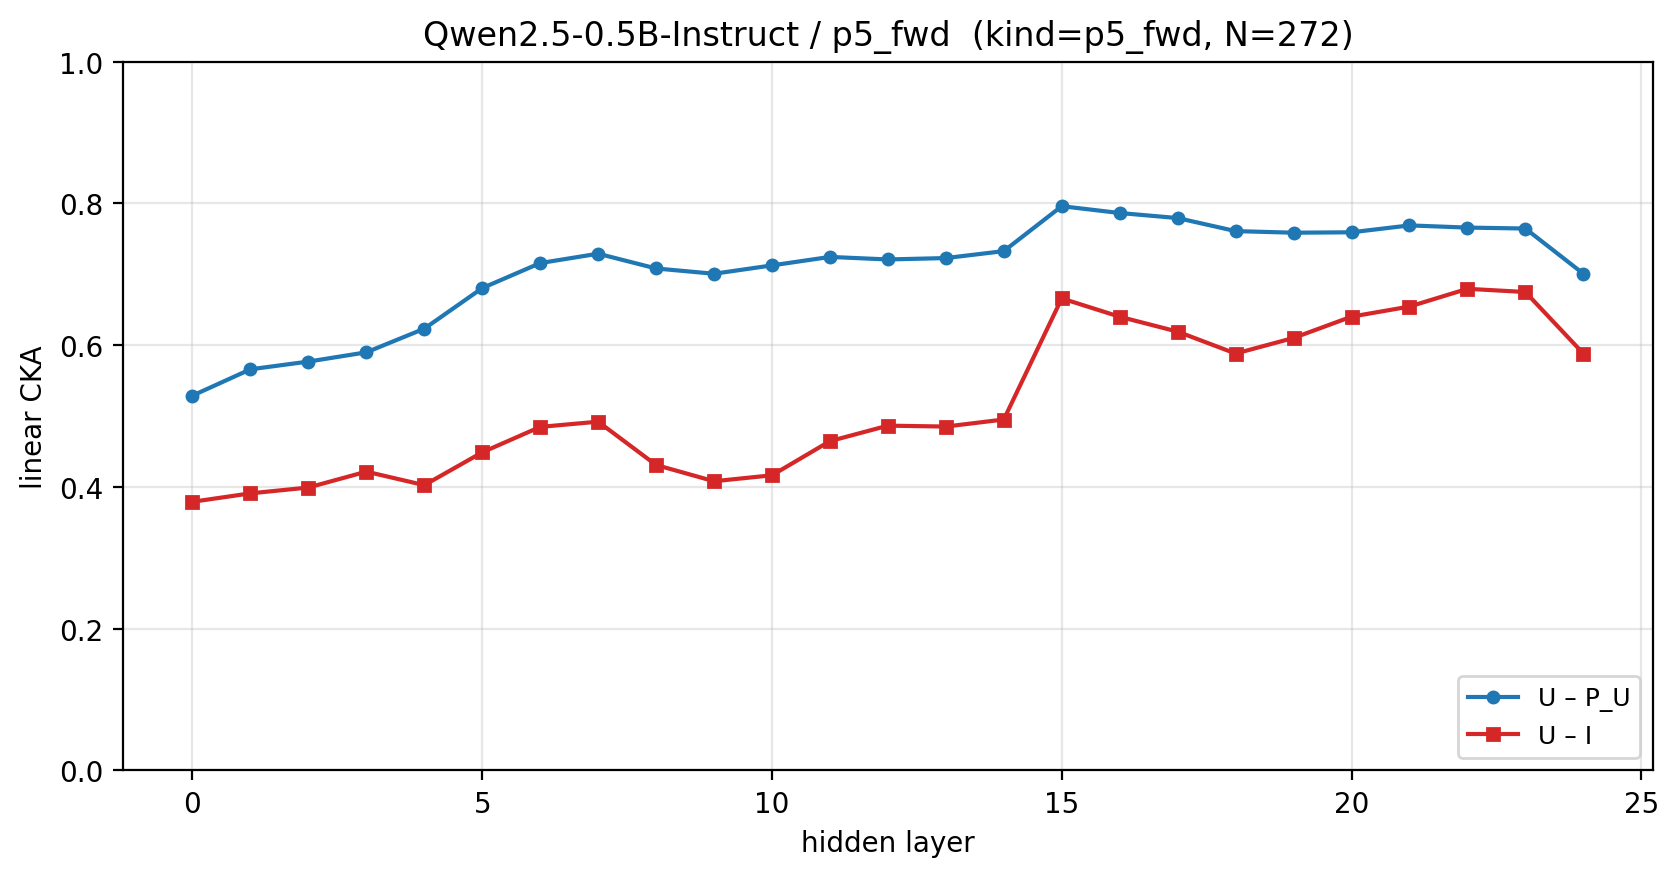
\includegraphics[width=0.95\textwidth,height=0.82\textheight,keepaspectratio]{experiments/2026-06-10_u_axes/plots/Qwen2.5-0.5B-Instruct_p5_fwd/u_axes_pPU_pI.png}
  \end{center}
\end{frame}

\begin{frame}{Qwen2.5-0.5B-Instruct\_p5\_fwd --- U–P\_U and U–I across layers}
  \small
  \textbf{Computation.} For each hidden layer $L$, build centered Gram matrices $K_X = X_c X_c^{\!\top}$ ($X_c = X - \bar X$) from the per-row bracket embeddings $X \in \{U, P_U, I\}$ over the $N$ stimuli. Plot linear CKA $\langle K_U, K_X\rangle_F / (\|K_U\|_F\,\|K_X\|_F)$ vs $L$ for each pair.
  \par\vspace{0.8em}
  \textbf{Interpretation.} How aligned the answer's geometry is with the paraphrase ($P_U$) and the inference ($I$) at each depth — higher means the two brackets reorder stimuli the same way. Where the two curves cross and how the gap evolves reveal when the model commits to a semantic vs pragmatic binding.
\end{frame}

\begin{frame}{Qwen2.5-0.5B-Instruct\_p5\_rev --- Layer×layer CKA: U vs P\_U and U vs I}
  \begin{center}
    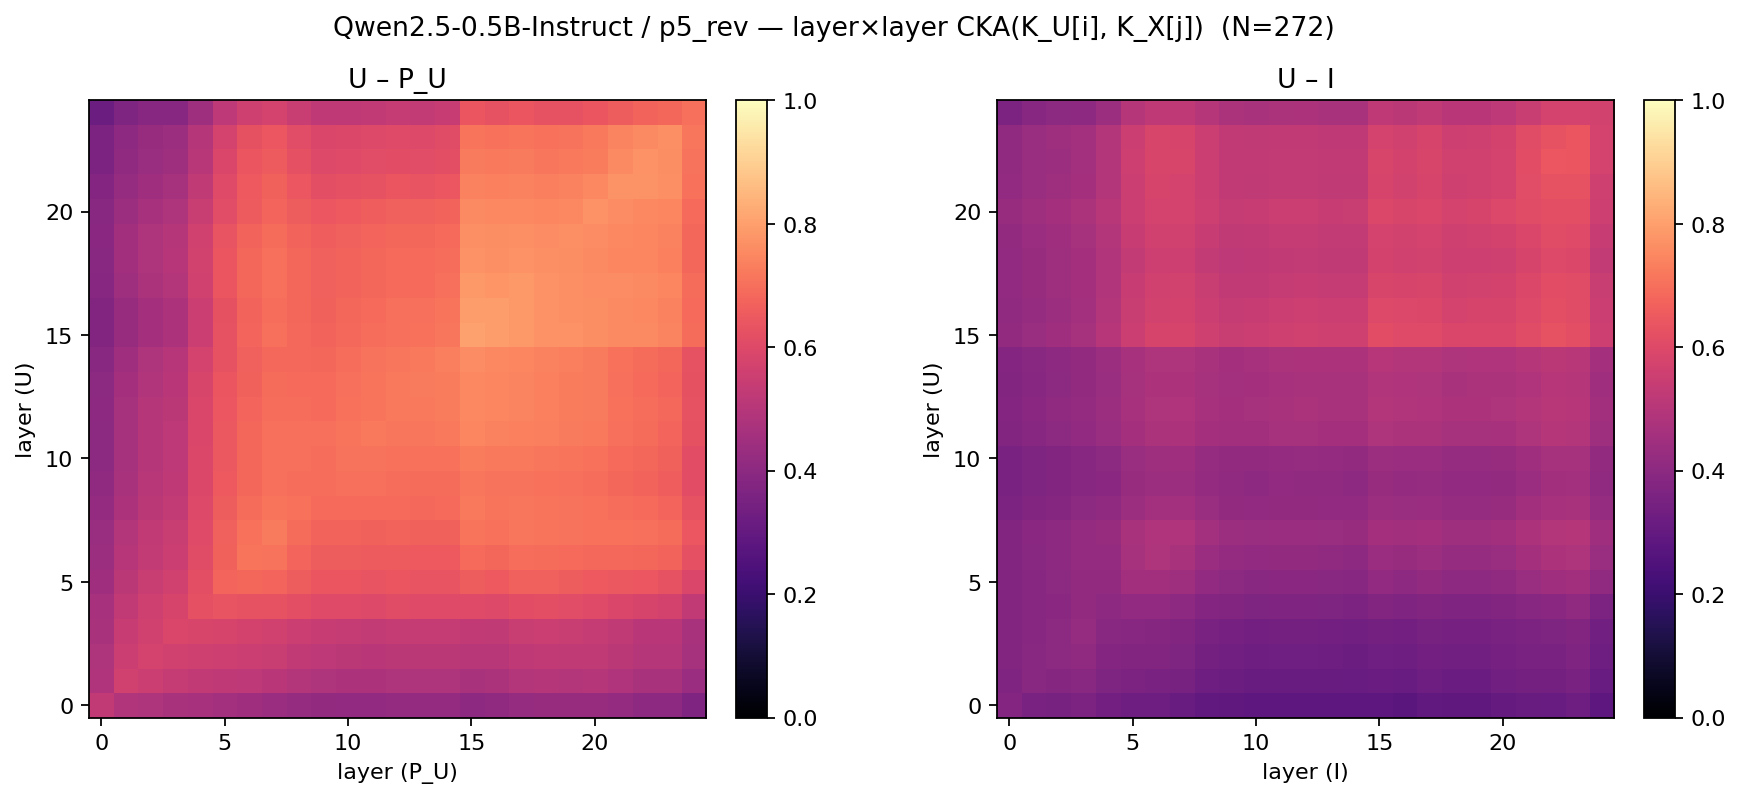
\includegraphics[width=0.95\textwidth,height=0.82\textheight,keepaspectratio]{experiments/2026-06-10_u_axes/plots/Qwen2.5-0.5B-Instruct_p5_rev/u_axes_layer_vs_layer.png}
  \end{center}
\end{frame}

\begin{frame}{Qwen2.5-0.5B-Instruct\_p5\_rev --- Layer×layer CKA: U vs P\_U and U vs I}
  \small
  \textbf{Computation.} Left: $M_{P_U}[i,j] = \mathrm{CKA}(K_U[i], K_{P_U}[j])$. Right: same with $K_I$. Diagonal cells reproduce the within-layer curves; off-diagonals are cross-depth alignment.
  \par\vspace{0.8em}
  \textbf{Interpretation.} Off-diagonal brightness flags delayed binding: $U$'s geometry at layer $i$ already matches the other bracket's geometry at a different layer $j$. Diagonal block structure suggests depth stages over which the alignment stabilizes.
\end{frame}

\begin{frame}{Qwen2.5-0.5B-Instruct\_p5\_rev --- U–P\_U and U–I across layers}
  \begin{center}
    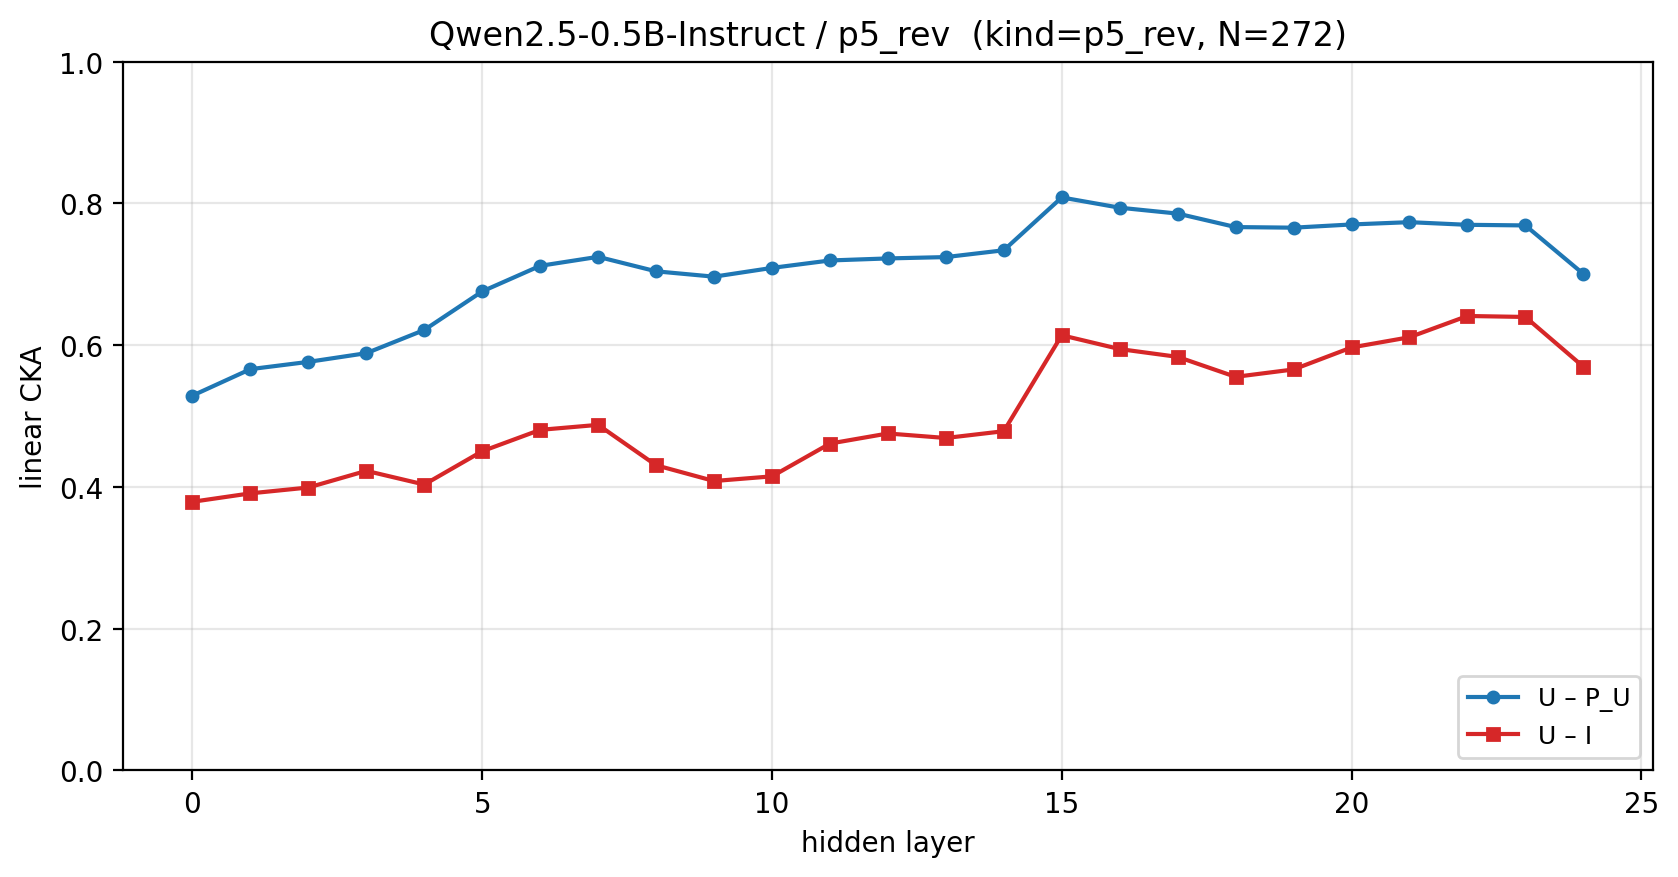
\includegraphics[width=0.95\textwidth,height=0.82\textheight,keepaspectratio]{experiments/2026-06-10_u_axes/plots/Qwen2.5-0.5B-Instruct_p5_rev/u_axes_pPU_pI.png}
  \end{center}
\end{frame}

\begin{frame}{Qwen2.5-0.5B-Instruct\_p5\_rev --- U–P\_U and U–I across layers}
  \small
  \textbf{Computation.} For each hidden layer $L$, build centered Gram matrices $K_X = X_c X_c^{\!\top}$ ($X_c = X - \bar X$) from the per-row bracket embeddings $X \in \{U, P_U, I\}$ over the $N$ stimuli. Plot linear CKA $\langle K_U, K_X\rangle_F / (\|K_U\|_F\,\|K_X\|_F)$ vs $L$ for each pair.
  \par\vspace{0.8em}
  \textbf{Interpretation.} How aligned the answer's geometry is with the paraphrase ($P_U$) and the inference ($I$) at each depth — higher means the two brackets reorder stimuli the same way. Where the two curves cross and how the gap evolves reveal when the model commits to a semantic vs pragmatic binding.
\end{frame}

\begin{frame}{Qwen2.5-0.5B-Instruct\_qwen\_mensaje --- Layer×layer CKA: U vs P\_U and U vs I}
  \begin{center}
    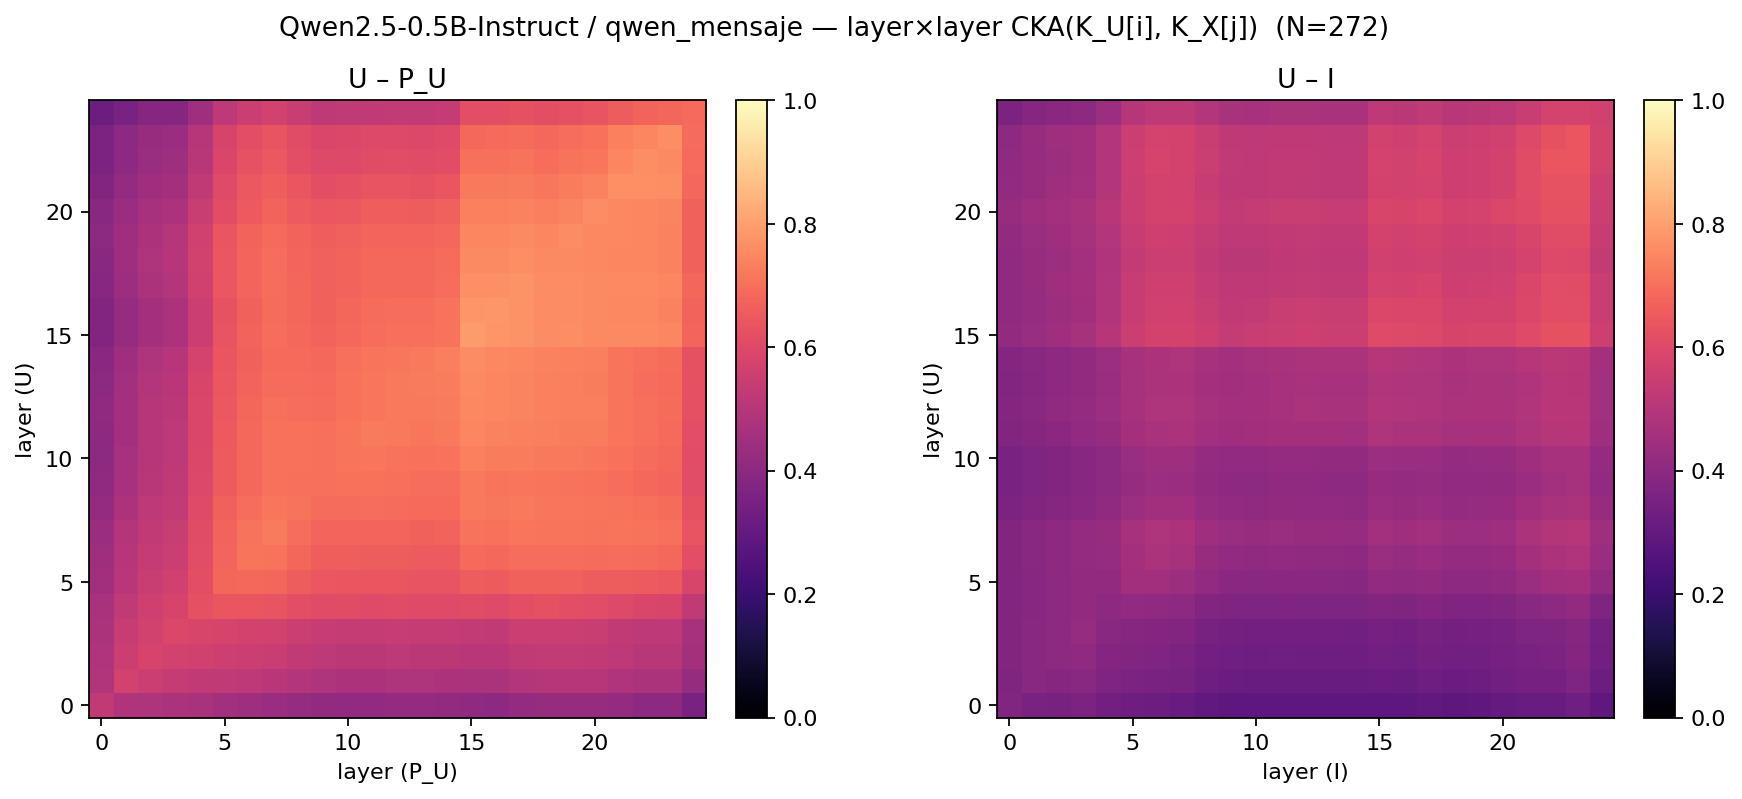
\includegraphics[width=0.95\textwidth,height=0.82\textheight,keepaspectratio]{experiments/2026-06-10_u_axes/plots/Qwen2.5-0.5B-Instruct_qwen_mensaje/u_axes_layer_vs_layer.png}
  \end{center}
\end{frame}

\begin{frame}{Qwen2.5-0.5B-Instruct\_qwen\_mensaje --- Layer×layer CKA: U vs P\_U and U vs I}
  \small
  \textbf{Computation.} Left: $M_{P_U}[i,j] = \mathrm{CKA}(K_U[i], K_{P_U}[j])$. Right: same with $K_I$. Diagonal cells reproduce the within-layer curves; off-diagonals are cross-depth alignment.
  \par\vspace{0.8em}
  \textbf{Interpretation.} Off-diagonal brightness flags delayed binding: $U$'s geometry at layer $i$ already matches the other bracket's geometry at a different layer $j$. Diagonal block structure suggests depth stages over which the alignment stabilizes.
\end{frame}

\begin{frame}{Qwen2.5-0.5B-Instruct\_qwen\_mensaje --- U–P\_U and U–I across layers}
  \begin{center}
    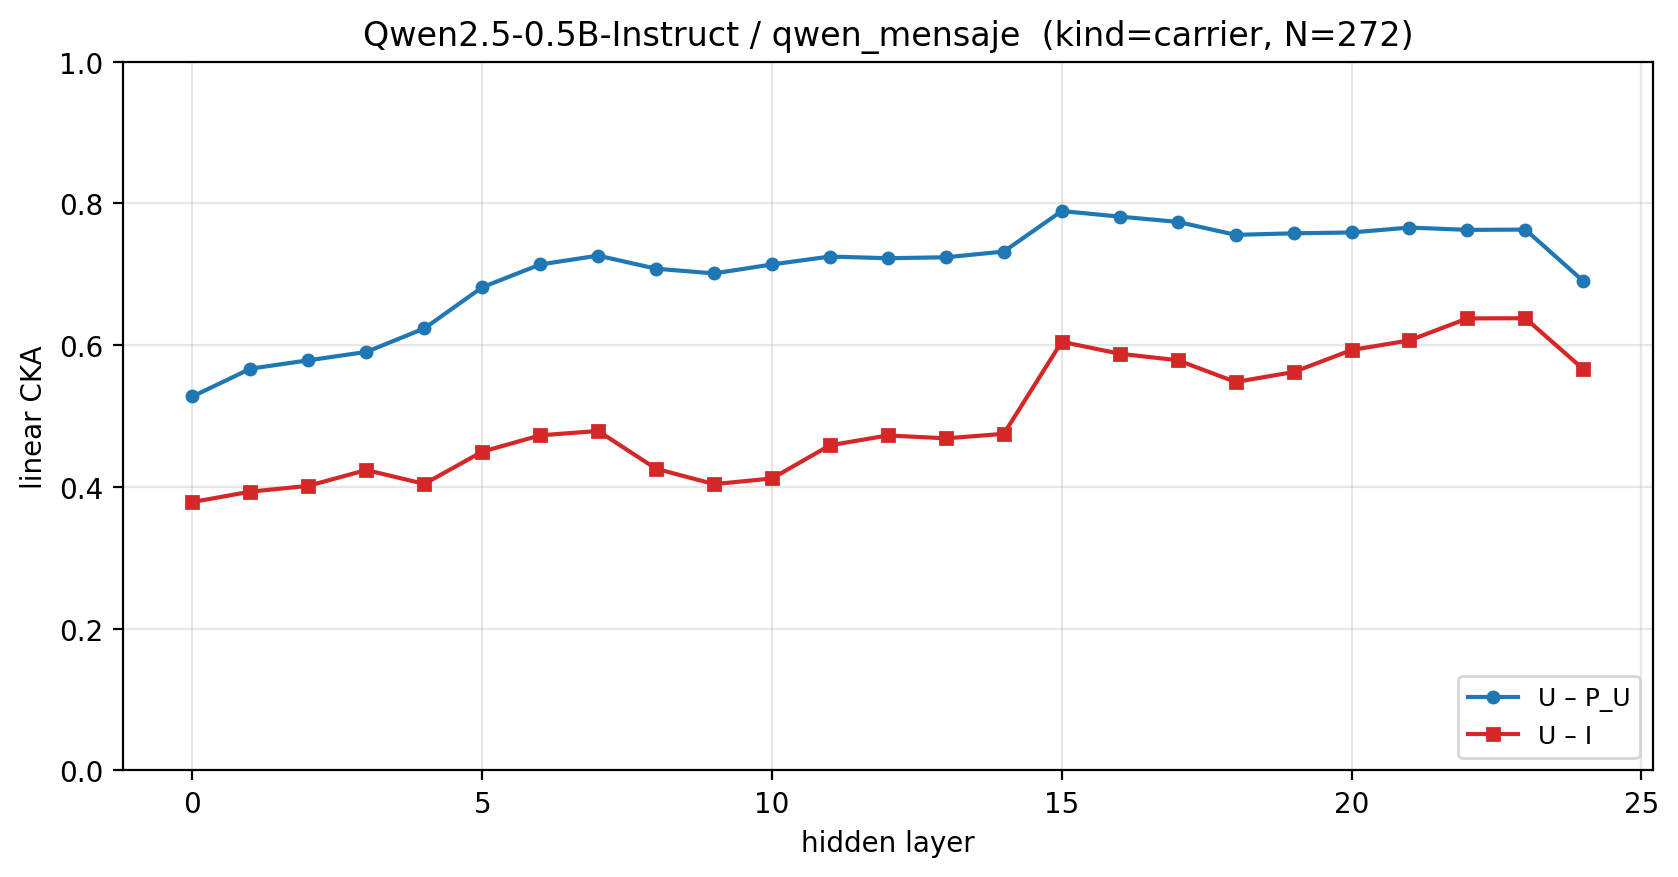
\includegraphics[width=0.95\textwidth,height=0.82\textheight,keepaspectratio]{experiments/2026-06-10_u_axes/plots/Qwen2.5-0.5B-Instruct_qwen_mensaje/u_axes_pPU_pI.png}
  \end{center}
\end{frame}

\begin{frame}{Qwen2.5-0.5B-Instruct\_qwen\_mensaje --- U–P\_U and U–I across layers}
  \small
  \textbf{Computation.} For each hidden layer $L$, build centered Gram matrices $K_X = X_c X_c^{\!\top}$ ($X_c = X - \bar X$) from the per-row bracket embeddings $X \in \{U, P_U, I\}$ over the $N$ stimuli. Plot linear CKA $\langle K_U, K_X\rangle_F / (\|K_U\|_F\,\|K_X\|_F)$ vs $L$ for each pair.
  \par\vspace{0.8em}
  \textbf{Interpretation.} How aligned the answer's geometry is with the paraphrase ($P_U$) and the inference ($I$) at each depth — higher means the two brackets reorder stimuli the same way. Where the two curves cross and how the gap evolves reveal when the model commits to a semantic vs pragmatic binding.
\end{frame}
